\documentclass[12pt]{article}
\usepackage[margin=0.75in]{geometry}
\geometry{a4paper}
\usepackage[T1]{fontenc} % Support Icelandic Characters
\usepackage[utf8]{inputenc} % Support Icelandic Characters
\usepackage{graphicx} % Support for including images
\usepackage{hyperref} % Support for hyperlinks
\usepackage{wrapfig}

\usepackage{algorithm}
\usepackage{algorithmicx}
\usepackage{listings}
\usepackage{color}
\usepackage{siunitx}

\usepackage[svgnames]{xcolor}

\usepackage{amsmath}
\usepackage{tikz}
\usetikzlibrary{arrows,automata}

\usepackage{tikz}
\usepackage{tikz-dependency}
\usepackage[spanish,es-noshorthands]{babel}

\usepackage[spanish]{babel}
\usepackage[latin1]{inputenc}
\usepackage[usenames]{color}

\definecolor{mGreen}{rgb}{0,0.6,0}
\definecolor{mGray}{rgb}{0.5,0.5,0.5}
\definecolor{mPurple}{rgb}{0.58,0,0.82}
\definecolor{backgroundColour}{rgb}{0.95,0.95,0.92}

\usepackage{xcolor}

\usepackage{listings}             % Include the listings-package
\lstdefinestyle{CStyle}{
    backgroundcolor=\color{backgroundColour},   
    commentstyle=\color{mGreen},
    keywordstyle=\color{blue},
    numberstyle=\tiny\color{mGray},
    stringstyle=\color{red},
    basicstyle=\footnotesize,
    breakatwhitespace=false,         
    breaklines=true,                 
    captionpos=b,                    
    keepspaces=true,                 
    numbers=left,                    
    numbersep=5pt,                  
    showspaces=false,                
    showstringspaces=false,
    showtabs=false,                  
    tabsize=2,
    language=C
}



%------------------------------------------------------------------
% TITLE
%------------------------------------------------------------------

\title{
\centerline{
    
\includegraphics[width=75mm]{unsa.png}}
    \vspace{0.5 cm}
        Teoría de la Computación - Laboratorio A
        \\
        \\
        \\
        \textbf{Práctica de Laboratorio #8} 
        \large  
        \\
        %SC-T-718-ATSR,Automatic Speech Recognition, 2019-1 
        %\\ 
        \small Universidad Nacional de San Agustín - Escuela Profesional de Ingeniería de Sistemas, Arequipa, Perú 
  }

\author{
    Carlos Alberto Mestas Escarcena
    \\
    \texttt{cmestas@unsa.edu.pe}
}

\date{Julio del 2020}

\begin{document}

\maketitle

El desarrollo de este informe se puede encontrar en el repositorio de \textcolor{blue}{
    \href{https://github.com/CarlosMestas/TC_A_7_Carlos_Mestas}{GitHub}}.
\\
\newline

Para el desarrollo de los ejercicios utilicé el siguiente código:

\begin{lstlisting}[language=bash,frame=single,style=CStyle,caption={le
%{
    #include "sintactico.tab.h"
    /*
    externt yylval
    */
%}
number [0-9]+
%%
{number}              {yylval = atoi(yytext); return (NUM);}
"\n"                  {return (EOL);}
.                     {return yytext[0];}
%%
int yywrap(){
    return 0;
}
\end{lstlisting}

\begin{lstlisting}[language=bash,frame=single,style=CStyle,caption={sintactico.y}]
%{
    #include <stdio.h>
    #include <stdlib.h>
    #define YYDEBUG 1
    extern int yylex(void);
    extern char *yytext;
    void yyerror(char* s);

%}
%token NUM
%token EOL

%left '+' '-'
%left '*' '/'

%%

stm_lst: stm stm_lst EOL 
       | stm EOL 
       ;

stm: exp ';'        {printf("= %d \n",$1);
                    exit(0);}
   ;

exp: exp '-' exp   { $$= $1 - $3;}
   | exp '+' exp   { $$= $1 + $3;}
   | exp '*' exp   { $$= $1 * $3;} 
   | exp '/' exp   { 
                      if($3!=0){
                        $$= $1 / $3;
                        }
                      else{
                        yyerror("No hay division entre 0");
                        $$ = 0;
                      }
                    }
   | exp '+' error  {printf("Error en la suma ... segundo termino\n");
                    yyerrok;
                    yyclearin;
                    }
   | error '+' exp  {printf("Error en la suma ... primer termino\n");
                    yyerrok;
                    yyclearin;
                    }
   | exp '-' error  {printf("Error en la resta ... segundo termino\n");
                    yyerrok;
                    yyclearin;
                    }
   | error '-' exp  {printf("Error en la resta ... primer termino\n");
                    yyerrok;
                    yyclearin;
                    }
   | exp '*' error  {printf("Error en la multiplicacion ... segundo termino\n");
                    yyerrok;
                    yyclearin;
                    }
   | error '*' exp  {printf("Error en la multiplicacion ... primer termino\n");
                    yyerrok;
                    yyclearin;
                    }
   | exp '/' error  {printf("Error en la division ... segundo termino\n");
                    yyerrok;
                    yyclearin;
                    }
   | error '/' exp  {printf("Error en la division ... primer termino\n");
                    yyerrok;
                    yyclearin;
                    }                 
   |  '(' exp ')'   { $$= $2;}
   |  NUM           { $$= $1;}
   ;
%%

void yyerror(char* s){
    printf("\tError sintactico: %s \n",s);
}

int main(int argc,char **argv){
    yydebug = 0;
    yyparse();
    return 0;
}
\end{lstlisting}

\section{Crear un ejemplo donde se use yyclearin}

Utilizamos el macro $yyclearin$ que nos sirve que el caso de que se encuentre un error, si nuestra gramática tiene una acción de reconocimiento asociada con \textbf{error} y con ello puede leer la siguiente entrada hasta que encuentre los siguientes datos seguros de ser válidos, si se desea que el analizador viejo deseche el viejo símbolo de búsqueda anticipada utilizaremos $yyclearon$.

\section{Se puede usar el token error en el analizador lexico, defina porque}

Si, por ejemplo si nosotros deseamos tokens de error en un nivel alto de la gramática este debe ir en el sintáctico, porque siempre tendremos una regla para que este pueda recuperarse, pero si nosotros deseamos descartar los errores lo más antes posible, antes de la recuperación puede ir en el léxico.

\section{Agregar una producción a la suma para producir varias sumas y agregar el token error junto con yyerrok}

\begin{figure}[h]
    \centering
    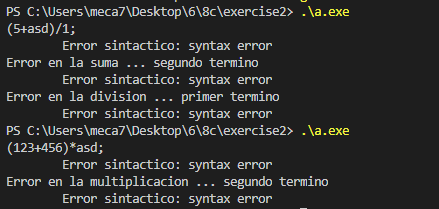
\includegraphics[width=0.8\textwidth]{images/CaptureC01.PNG}
    \caption{Ejemplo de compilación}
\end{figure}

    



\end{document}